% !TeX spellcheck = en_GB
\chapter{Concept} % Lösungsentwurf 
\epigraph{Perfection (in design) is achieved not when there is nothing more to add,\\but rather when there is nothing more to take away.}{Antoine de Saint-Exupery}

% (Lösungsvarianten und deren Beurteilung, Variantenentscheid, Konzept, Entwurf)
% See arch. decisions

\section{Architecture}\label{sec:architecture}
% - Architekturdiagramme inkl. Layering (C4, UML)
% - mit Entscheidungen und begründung
% - wie Qualitätsattribute sichergestellt wurden
% - Beschreibung des Entwurfs (welche Experimente/Tests wurden durchgeführt? welche Lösungsoptionen wurden verworfen?)
% - Entwurf Benutzerschnittstelle

In this chapter, we present the architecture and fundamental architectural decisions of the \gls{xmpp-grid-broker} application.
All architectural decisions we took are fully documented in Appendix~\fullref{sec:architectural-decisions}.

We illustrate the concepts and structures using the \emph{C4 Model for Software Architecture}~\cite{c4-model}.

\subsection{Actors and Context}

The context diagram pictured in Figure~\ref{fig:architecturecontext} shows the surrounding systems and actors that are given for the \gls{xmpp-grid-broker}, as described in the \nameref{sec:task-description}.

One or more administrators manage the \gls{xmpp-grid} by adding or removing \glspl{platform} and configuring \glspl{topic}.
To minimize the required work and reduce the error-proneness, they interact with the \gls{xmpp-grid-broker}, whose implementation is the primary goal of this thesis.

The \gls{xmpp-grid-broker} configures the \gls{xmpp-grid}, which consists of a \gls{controller} and \glspl{platform}.

\begin{figure}[h]
\centering
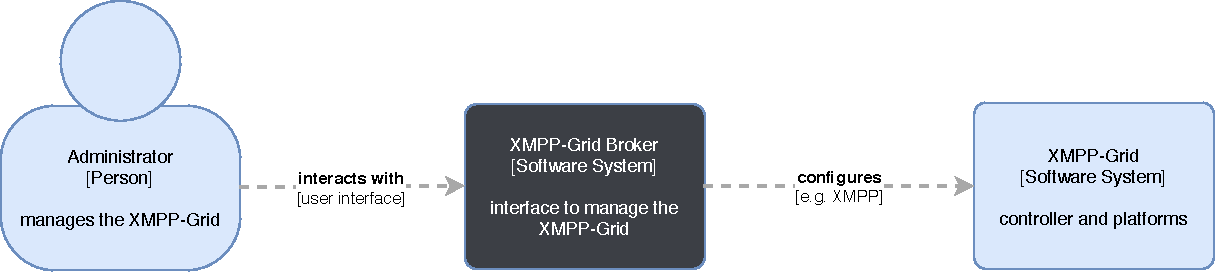
\includegraphics[width=\linewidth]{resources/architecture_context}
\caption[Architecture context diagram]{Architecture diagram showing the context of the \gls{xmpp-grid-broker} application.}
\label{fig:architecturecontext}
\end{figure}


\subsection{Architectural Style and Platform}

To implement the \gls{xmpp-grid-broker}, we evaluated three possible architecture styles:\hfill\\
An \gls{xmpp} server plug-in (e.g. extension for the Openfire \gls{xmpp} server), an implementation with the Jabber Component Protocol~\cite{xep-0114} or an implementation acting as a regular \gls{xmpp} client ("bot").

We decided to build an \gls{xmpp} client/bot, because it is not coupled to a specific \gls{xmpp} server as a server plug-in and, in contrast to the \gls{xmpp} component, supports a strong authentication mechanism with \gls{sasl}.

The full decision argument is documented in Appendix~\fullref{sec:architectural-decisions}.

\subsubsection{Platform}

The proposed \gls{xmpp} client might be implemented in different ways: as rich client application with a command line or graphical interface as illustrated in Figure~\ref{fig:architecturecontainerrichclient}, or in the form of a web application, illustrated in Figures~\ref{fig:architecturecontainerwebapplication} and \ref{fig:architecturecontainerwebproxy}.

\subsection{Rich Client Application}

In contrast to a rich client application, a web application has the significant advantage to be easily installable and upgradable with minimal requirements on the user's side (i.e. only requires a web browser to be executed).
Therefore, we decided to implement the \gls{xmpp-grid-broker} as web application.

\begin{figure}[h]
\centering
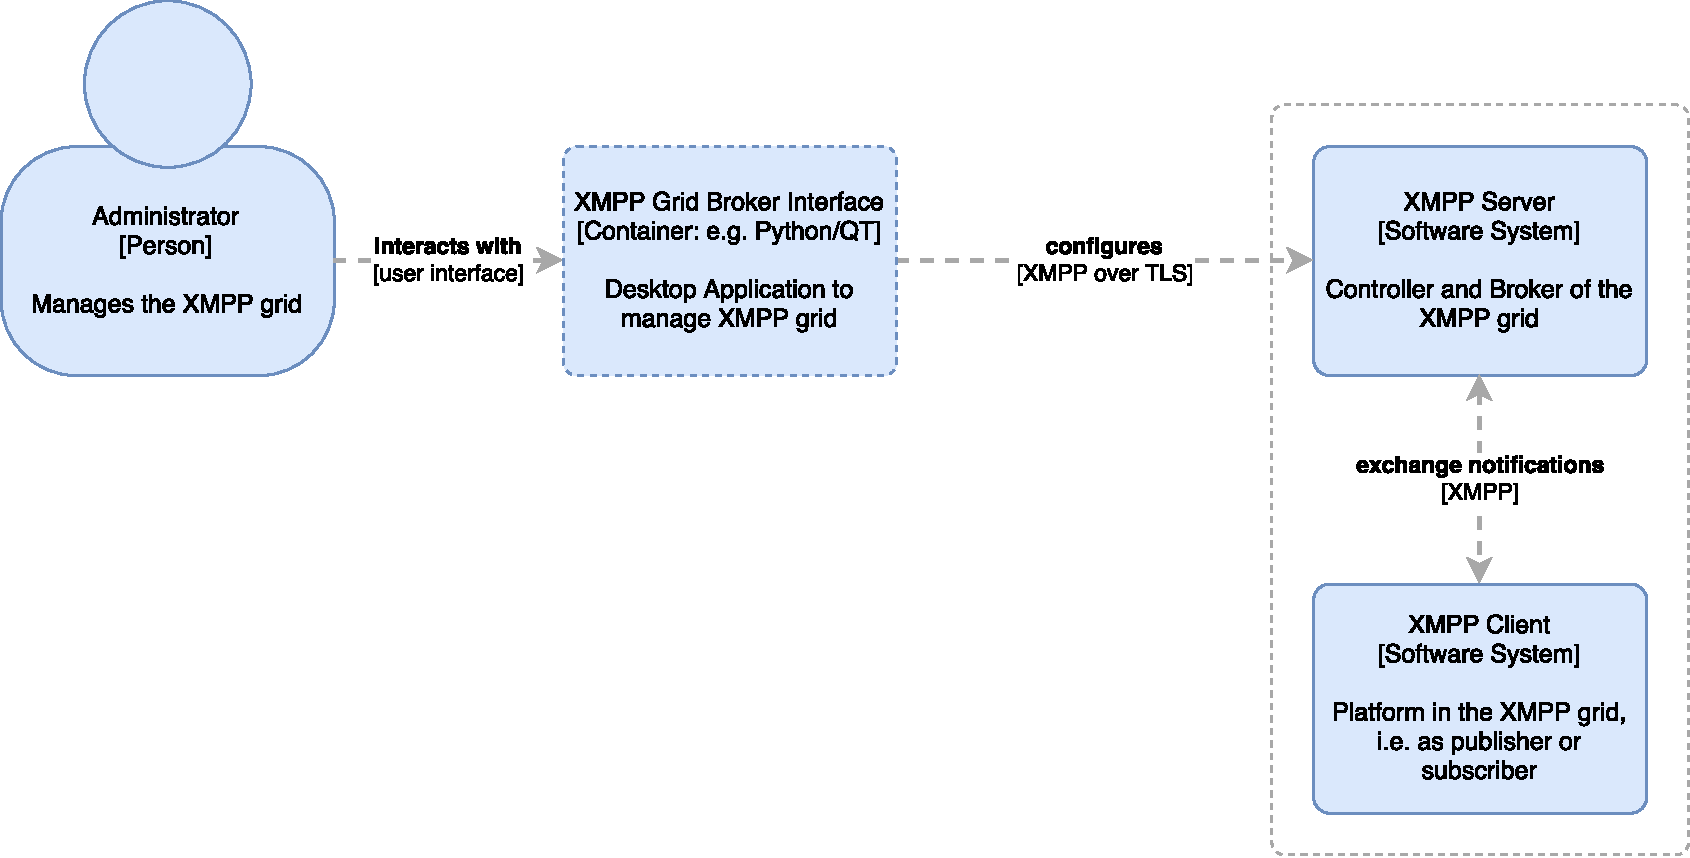
\includegraphics[width=0.7\linewidth]{resources/architecture_container_rich_client}
\caption[Architecture container diagram: Rich client]{Architecture container diagram showing a possible rich client architecture.}
\label{fig:architecturecontainerrichclient}
\end{figure}

\subsection{Web Application Topology}

To manage the \gls{controller} from our interface, we considered the implementation of either directly connecting to the \gls{xmpp} server over WebSockets~\cite{rfc7395} or HTTP (BOSH~\cite{xep-0124}), or to communicate indirectly with the \gls{xmpp} server via custom web API proxy.
These topologies are illustrated in Figure~\ref{fig:architecturecontainerwebapplication} and Figure~\ref{fig:architecturecontainerwebproxy}.

\begin{figure}[h]
\centering
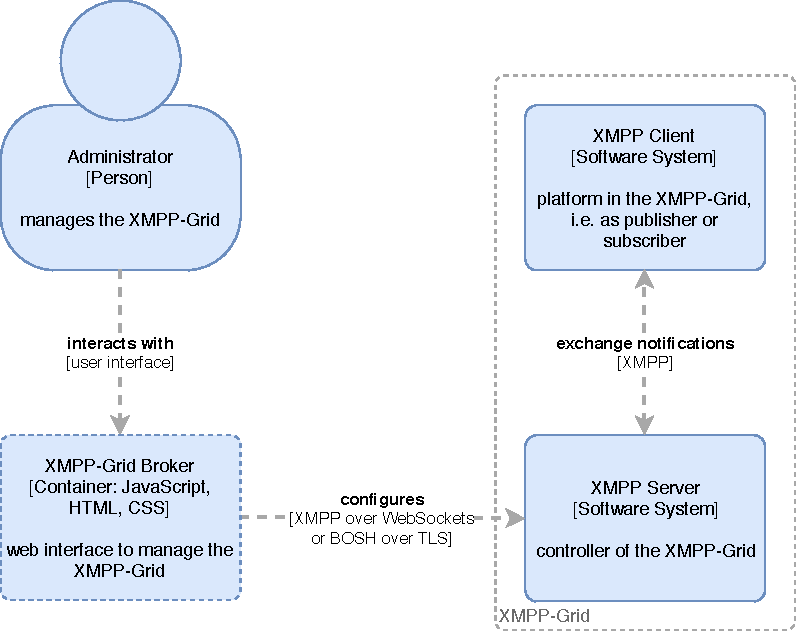
\includegraphics[width=0.7\linewidth]{resources/architecture_container_webapplication}
\caption[Architecture container diagram: Web application]{Architecture container diagram showing the web application topology with WebSockets or BOSH.}
\label{fig:architecturecontainerwebapplication}
\end{figure}

\subsubsection{Web API Proxy}

A web API proxy could be realised with a custom browser-to-proxy protocol, as implemented in the \gls{xmpp}-FTW JavaScript library\footnote{\url{http://docs.xmpp-ftw.org/}}.
However, this approach leads to a high coupling between a concrete library and the web application.

Another approach would be the implementation of a custom WebSocket-to-\gls{xmpp} Proxy, which allows connecting to \gls{xmpp} servers that do not support WebSockets or BOSH.
If such a proxy is implemented transparently, the client is not aware of the server limitations.
Therefore, the client implementation is no different from direct communication with an \gls{xmpp} server.

As the `\gls{xmpp} over WebSocket' protocol differs from the normal \gls{xmpp} protocol, a transparent proxy implementation would inevitably need to hold the connection state and implement custom keep-alive mechanisms~\cite{rfc7395}.

\begin{figure}[H]
\centering
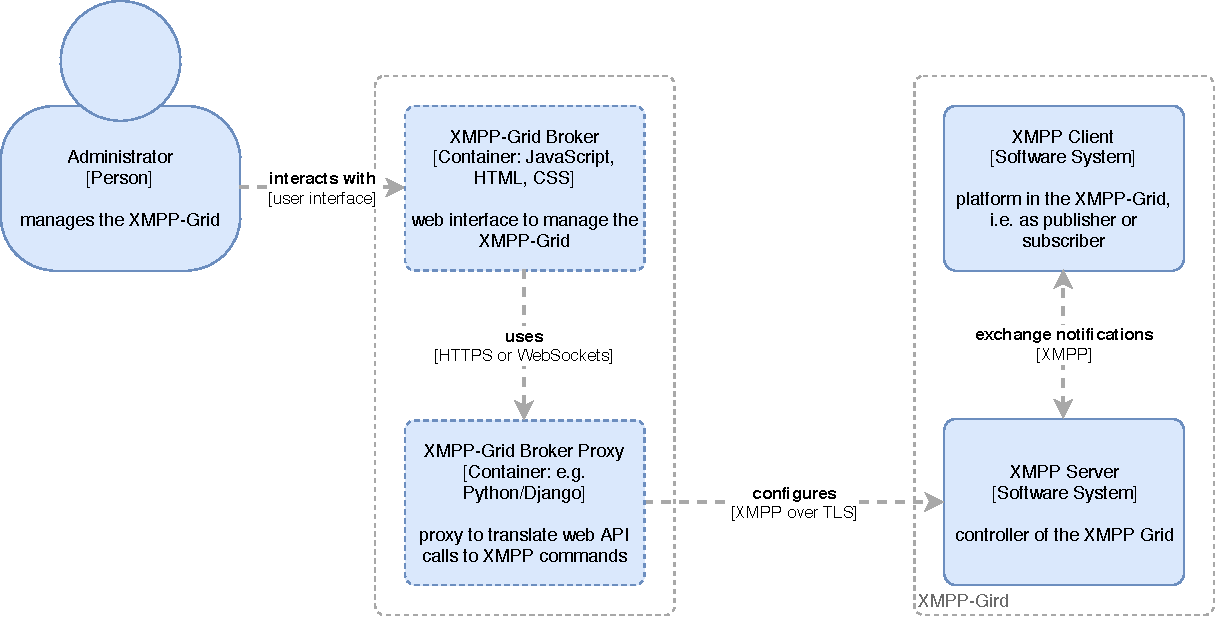
\includegraphics[width=0.8\linewidth]{resources/architecture_container_proxy}
\caption[Architecture container diagram: Web proxy]{Architecture container diagram showing the web API proxy topology.}
\label{fig:architecturecontainerwebproxy}
\end{figure}

\subsubsection{Implemented Web Application Topology}\label{sec:implemented-web-application-topology}

As described in the according architectural decision (see Appendix~\ref{sec:architectural-decisions}), we decided on the direct connection via WebSockets, if possible with a fallback to BOSH.
This topology simplifies the implementation and deployment of the application in comparison to a web API proxy.
WebSockets offer stateful TCP-sockets to exchange data with the \gls{xmpp} server in contrast to BOSH, which uses HTTP long polling to emulate a bidirectional stream and is, therefore, less efficient~\cite{xep-0124}.

To increase the \gls{xmpp} server security, an HTTP reverse proxy (e.g.\ nginx\footnote{\url{https://nginx.org/}}) between the client and the \gls{xmpp} server might be added as shown in Figure~\ref{fig:architecturecontainerweb-http-proxy}.
The reverse proxy might also be used to serve the web application and provide authentication (see Section~\ref{sec:authentication-and-connection-security}) and security features (see Section~\ref{sec:ops-security}).

\begin{figure}[H]
    \centering
    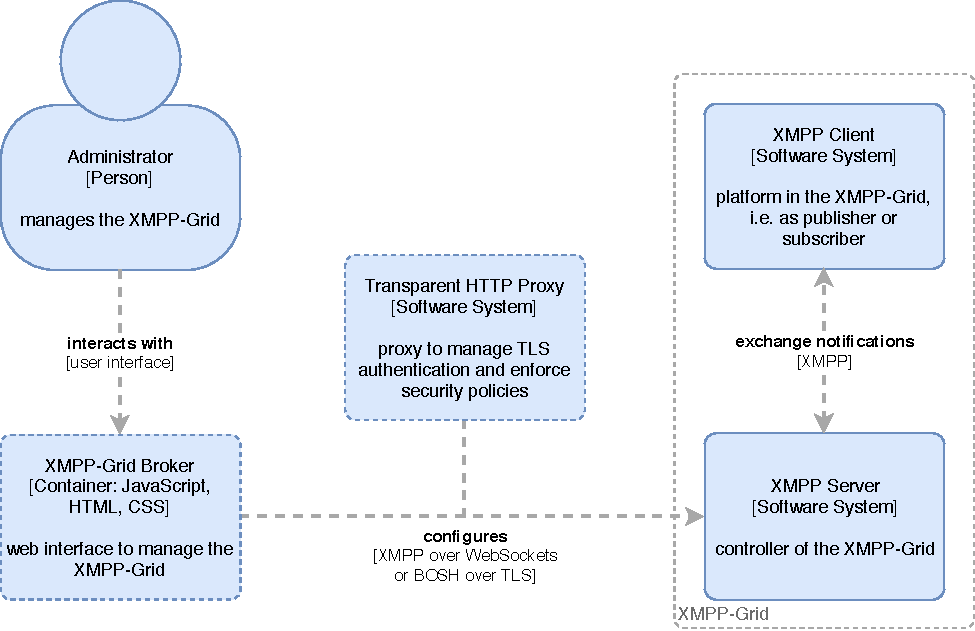
\includegraphics[width=\linewidth]{resources/architecture_container_webapplication_with_http_proxy}
    \caption[Architecture container diagram: Web application with transparent proxy]{Architecture container diagram showing the implemented web application topology.}
    \label{fig:architecturecontainerweb-http-proxy}
\end{figure}
  

\subsection{Authentication and Connection Security}\label{sec:authentication-and-connection-security}

\gls{xmpp} uses \gls{sasl} as authentication mechanism~\cite{rfc6120}.
To authenticate against the \gls{xmpp-grid} \gls{controller}, we decided to use the \gls{sasl-external}~\cite{rfc4422} mechanism whenever possible to authenticate the client.

We decided against the alternative \gls{sasl} authentication method, \gls{sasl-scram}~\cite{rfc7677}, that is also recommended by in the \gls{xmpp-grid} standard~\cite{ietf-mile-xmpp-grid-05}.
As described in the corresponding architectural decision (Appendix~\ref{sec:architectural-decisions}), the main reason for \gls{sasl-external} is its higher level of security and and its relatively simple scaling capabilities.

\gls{sasl-external} implies that the authentication takes place on a lower layer than the actual \gls{xmpp} protocol. In our case, this implies authentication over \gls{tls}, i.e.~X.509 end-user certificates as specified in RFC6120~\cite{rfc6120}.

Currently, not all \gls{xmpp} servers that implement BOSH and Websockets also implement \gls{sasl-external} with \gls{tls} authentication
(e.g.\ Openfire currently supports \gls{tls} authentication with BOSH but not with Websockets\footnote{\url{https://github.com/igniterealtime/Openfire/blob/02c22e/src/java/org/jivesoftware/openfire/websocket/OpenfireWebSocketServlet.java}}).
To circumvent this limitation, a HTTP reverse proxy as described in Section~\ref{sec:implemented-web-application-topology} might be used, which handles the \gls{tls} authentication.

\subsubsection{Concurrency, Scalability and Performance}

As presented in the architecture above, the \gls{broker} application communicates directly from the user's web browser with the \gls{xmpp} server.
By adopting this approach, the main scalability concern is on the \gls{xmpp} server.
This approach is also in alignment with the \gls{xmpp} philosophy to move as much complexity as possible on the server \cite{definitive-guide-xmpp}.

Concurrency and scalability are the responsibility and speciality of the underlying \gls{xmpp} server and therefore not directly relevant for the \gls{broker} application \cite{definitive-guide-xmpp}.

Regarding performance, the network is the primary source of potential slowdowns.
The \gls{xmpp-grid} \gls{broker} must reduce the number of requests needed to a minimum and whenever possible execute requests in parallel.
Additionally, the initial loading time of the application can be optimised.

A potentially used reverse proxy must be scaled with the number of administrators.
As this number is usually rather small, no extra effort is usually required.

\section{Wireframes}

We created wireframes for most screens to visualise the initial set of user stories.
They helped us to find missing requirements, most notably the support of collections.
All wireframes are listed in Appendix~\fullref{sec:wireframes}.

\section{Security Considerations}\label{sec:security-considerations}

Regarding only the \gls{xmpp-grid-broker} application, there are three primary attack vectors:

\begin{description}
    \item[Client-side attacks,] e.g. via web browser, web browser extension or malicious software on the client operating system.
    \item[Web server attacks,] e.g. misconfiguration or insufficient hardening.
    \item[\gls{xmpp} server attacks,] e.g. misconfiguration or insufficient hardening.
\end{description}

Details on all attack vectors are discussed in the following sections.

\subsection{The \gls{xmpp} Protocol}

An in-depth security analysis of the \gls{xmpp} protocol is beyond the scope of this thesis.
A detailed discussion of security concerns can be found in the \gls{xmpp} specification~\cite{rfc6120} and most XEPs~\cite{xep-0060}\cite{xep-0248}.
In this section, we highlight the most crucial security concerns relevant to this thesis.

\subsubsection{Transport Security}

\gls{xmpp} reuses many established and standardised mechanisms to improve the protocol security.
By layering protocols in a strict manner (\gls{xmpp} with \gls{sasl} over \gls{tls} over TCP), many attack scenarios such as replaying or eavesdropping are minimised.
The protocol also requires clients and servers to validate the certificates of the other party.~\cite{rfc7590}\cite{rfc6120}

\subsubsection{Protocol}

Since \gls{xmpp} is based on XML, it inherits some of its security implications.
\gls{xmpp} prohibits some XML features such as comments and external entity references which mitigate common attacks.~\cite{rfc6120}

The protocol itself cannot mitigate attacks where an attacker gains access to account credentials.
To reduce the risk of these attack vectors best practices such as storing certificates and passwords securely must be followed.

\subsubsection{PubSub Collection Nodes}

The use of PubSub Collection Nodes~\cite{xep-0248} can leak private data if not configured properly.
Administrators must take great care when configuring collection nodes.
The \gls{xmpp-grid-broker} should support administrators to detect such data leaks.

\subsection{Client Security}

Because the web gives rise to many potential security concerns, above all a modern web browser is critical for client security.
Legacy web browsers can not provide an adequate level of security.~\cite{firefox-update-security}

Most web browser support extension mechanisms which have rather significant capabilities.
The usage of untrusted or uncertified browser extensions is strictly discouraged.~\cite{browser-extension-security}

The same applies to the client operating system and all software installed on clients.

\subsubsection{Authentication and Authorisation}

Regarding authentication and authorisation, the \gls{xmpp} server does most of the heavy lifting such as storing passwords and validating certificates.
On the client side, the web browser does most of that work too (i.e. validating certificates).

The responsibility of our client implementation is to establish a secure channel to the \gls{xmpp} server and warn the user if a problem occurs during this process (e.g. invalid server certificate).

\subsubsection{Angular Framework}

Using the Angular framework impacts client security significantly.
Angular is built with security in mind and is adopted in the industry in security-relevant environments.
Therefore, Angular receives frequent security updates and is well tested.
It's unlikely that a similar security level might be reached with plain JavaScript in a reasonable implementation timespan.

On their project website, Angular recommends the following three best practices regarding security~\cite{angular-security}.

\begin{itemize}
    \item Keep up with the latest Angular library releases.
    \item Don't modify your copy of Angular.
    \item Avoid Angular APIs marked in the documentation as ''Security Risk''.
\end{itemize}

We can ensure the latter two by making them acceptance criteria.
Keeping current with the latest Angular releases is harder, as our work on this project is limited.
To ensure that future updates can easily be applied we deviate as little as possible from the standard angular setup (e.g. by not ejecting the Webpack configuration\footnote{\url{https://github.com/Angular/Angular-cli/wiki/eject}}).

Keeping Angular up-to-date is of paramount importance as potential vulnerabilities (e.g. XSS) can be exploited if not patched.

\subsubsection{Angular Content Security}

Except for \glspl{persisted-item}, no \gls{xmpp} content is displayed directly but serves as the basis for rendered HTML components.
To protect against malicious payloads, the received XML messages must be validated before their usage.

\Glspl{persisted-item} can contain arbitrary content and must therefore be escaped before rendering to prevent Cross-Site Scripting (XSS) attacks.

Angular supports these measures by treating all values (except Angular templates) as untrusted by default.
To prevent user-generated data to influence Angular templates, the offline template compiler is used. To fully utilise the security measures provided by Angular, their APIs must be used at all times instead of direct use of the DOM-APIs.~\cite{angular-security}

Using Content-Security-Policy (CSP) provides additional XSS-protection mechanisms \cite{w3c-csp}.
The \gls{xmpp-grid-broker} should document an appropriate CSP that must be supported in a production environment.

\subsection{Server Security}

\subsubsection{Authentication and Authorisation}

The \gls{xmpp} server implements most of the authentication and authorisation mechanisms used in an \gls{xmpp-grid-broker} implementation, such as storing passwords and validating certificates.

If BOSH or WebSockets are used, the \gls{xmpp} server should supports most HTTP security features as listed in Section~\ref{sec:web-server}. Additionally, the origin of WebSockets and BOSH requests must be verified (by either the \texttt{Origin}-Header or CORS support.~\cite{rfc6455}\cite{cross-origin-resource-sharing}

The web server hosting the client application has no active authentication or authorisation responsibility, except to ensure the integrity and authenticity of the application, i.e. by using \gls{tls}.

\subsubsection{Web Server}\label{sec:web-server}

To minify security concerns on the server side, we decided to keep the application files static (See \fullref{sec:architectural-decisions}).
This allows operators to use any standard web server (e.g. NGINX, Apache, etc.) to serve the client.
Securing such standard web servers is common knowledge for operators and is beyond the scope of this analysis.

In addition to these general best practices, we explicitly recommend the following security measures to improve client security:

\begin{itemize}
    \item Enable Content Security Policy (CSP)~\cite{w3c-csp}.
    \item Use secure \gls{tls} configurations such as secure Cipher Suites, strictly Honor Cipher Order, HSTS, HPKP and OCSP Stapling\footnote{\url{https://wiki.mozilla.org/Security/Server_Side_TLS}}.
\end{itemize}


\subsubsection{\gls{xmpp} Server}

\gls{xmpp} server security depends on the chosen implementation and the application domain.
Discussing \gls{xmpp} server security in detail is beyond the scope of this thesis.
Operators should adhere to the security recommendations of their \gls{xmpp} server vendor and follow general security best practices as outlined by the \gls{xmpp-grid} standard~\cite{ietf-mile-xmpp-grid-05}.

\section{Security Risk Mitigation}\label{sec:security-risk-mitigation}

To mitigate the security risks as discussed in Section~\ref{sec:security-considerations}, the measures as described in the following subsections are implemented.

\subsection{Development}

\begin{enumerate}
    \item Conduct Code Reviews for all newly added code using GitHub pull requests and a security checklist (See next section)
    \item Conduct an architectural analysis with an industry expert\footnote{Was carried out on 2018-04-16, see \fullref{sec:meeting-minutes}.}
    \item Automate build and release processes to minimise the time required to patch.
    \item Stay as close to the default Angular setup to simplify further updates
    \item Avoid additional third-party dependencies whenever possible
\end{enumerate}

\subsection{Client Security Checklist}
\begin{itemize}
    \item The latest Angular-version is used
    \item No customizations are made to the Angular version
    \item No direct access to DOM-APIs
    \item APIs marked in the documentation as ``Security Risk'' are \emph{not} used
    \item No usage of any Methods starting with \texttt{bypassSecurityTrust}.
    \item The client is fully Content Security Policy compliant
    \item The client is fully Same Origin Policy (SOP) / Cross-Origin Resource Sharing (CORS) compliant
    \item Only compile templates offline using the offline template compiler.
    \item User input is always escaped using the mechanisms provided by the framework (eg. Angular Forms)
    \item \gls{xmpp} \glspl{message} are validated to contain only the specified result-types
\end{itemize}

\subsection{Operations Security}\label{sec:ops-security}


Administrators must configure the surrounding systems correctly to mitigate certain security risks.
To support administrators, we recommend the following measures.

\subsubsection{Content Security Policy}

The Content Security Policy (CSP) helps to mitigate certain types of attacks such as Cross Site Scripting (XSS) as a second line of defence \cite{w3c-csp}.
The recommended values are directly documented in the project source code repository.

\subsubsection{Verify Origin}
The \gls{xmpp} server should be configured to only accept WebSockets/BOSH connections from the origin of the \gls{xmpp-grid-broker} application.
The `Origin' Header sent by the web browser must match the domain on which the \gls{xmpp-grid-broker} application is hosted.
Otherwise, connection requests must be ignored.
If an \gls{xmpp} server does not support this feature, a proxy server should be used to verify the `Origin' header.
In the provided development setup, this security feature is not implemented.
